\documentclass[a4paper, 12pt]{article}
\usepackage{titling}
\usepackage{array}
\usepackage{booktabs}
\usepackage{enumitem}
\usepackage{graphicx}
\usepackage{subfigure}
\usepackage{hyperref}
\usepackage{amssymb}
\usepackage{listings}
\setlength{\heavyrulewidth}{1.5pt}
\setlength{\abovetopsep}{4pt}
\setlength{\parindent}{0pt}
\graphicspath{{.}}

\usepackage[margin=1in]{geometry}

% Must be after geometry
\usepackage{fancyhdr}
\pagestyle{fancy}
\fancyhf{}
\rhead{ECTA Homework 2}
\cfoot{\thepage}

\setlength{\droptitle}{-5em}

\title{Evolutionary Computation Theory and Application  \\
				Assignment 2: Traveling Salesman Problem}
\author{Arun Prabhu, Dharmin B.}
\date{\today{}}

\begin{document}

\maketitle


\section{Parameter used for solution}

\begin{table} [h!]
	  \centering
    \begin{tabular}{|l|c|}
    \hline
    \textbf{Parameter} & \textbf{Value}   \\\hline
    Population size & 50 \\\hline
    Crossover Rates &  0.01, 0.1, 0.99, \textbf{0.98}\\\hline
    Mutation Rates & 0.01, 0.1, 0.99, \textbf{0.25}\\\hline
    Repetitions & 30 \\\hline
    Generations & 1000 \\\hline
    Average best fitness		 & 59.2327 \\\hline
    Best fitness & 55.8960 \\\hline
    Plot & Figure~\ref{fig:plot} and ~\ref{fig:plotAndMap1000}\\\hline
    \end{tabular}
\caption{Parameters for Experiments}
\label{table:defparams}
\end{table}

\begin{table}[h!]
    \centering
    \label{tab:label}
    \begin{tabular}{|l|c|}\hline
        \textbf{Parameter} & \textbf{Value} \\\hline
        Population size & 100 \\\hline
        Fitness & 50.7048 \\\hline
        Generations & 3000 \\\hline
        Crossover rate & 0.99 \\\hline
        Mutation rate & 0.1 \\\hline
        Map image & Figure~\ref{fig:absBest} and ~\ref{fig:plotAndMap3000} \\\hline
    \end{tabular}
    \caption{Parameters for Absolute best result}
\end{table}
\newpage
\section{Results}

\begin{figure}[h!]
  \centering
  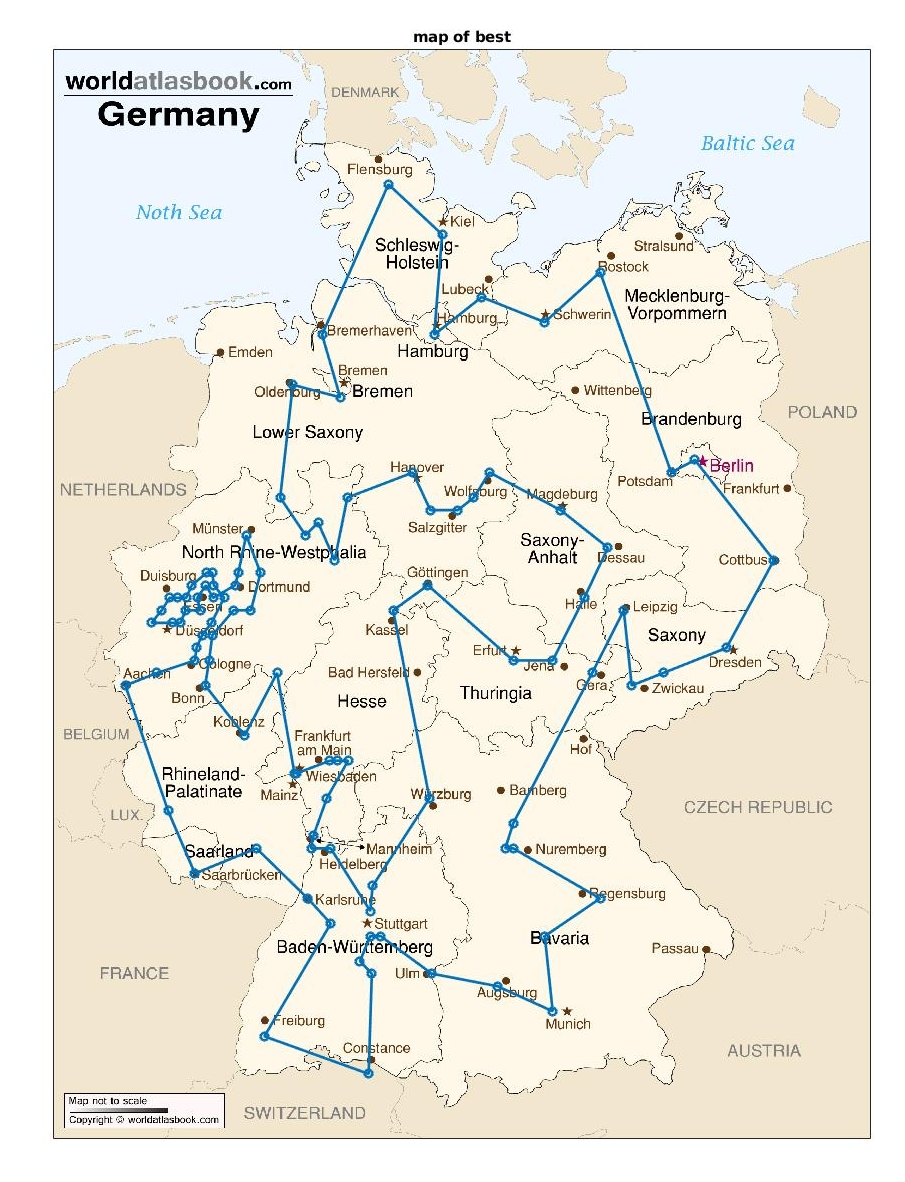
\includegraphics[width=1.0\textwidth]{images/BestPath_ultimate.jpg}
    \caption{Absolute best map \label{fig:absBest}}
\end{figure}

\newpage
\subsection{Different crossover rates}

\begin{figure}[ht!]
	\centering
	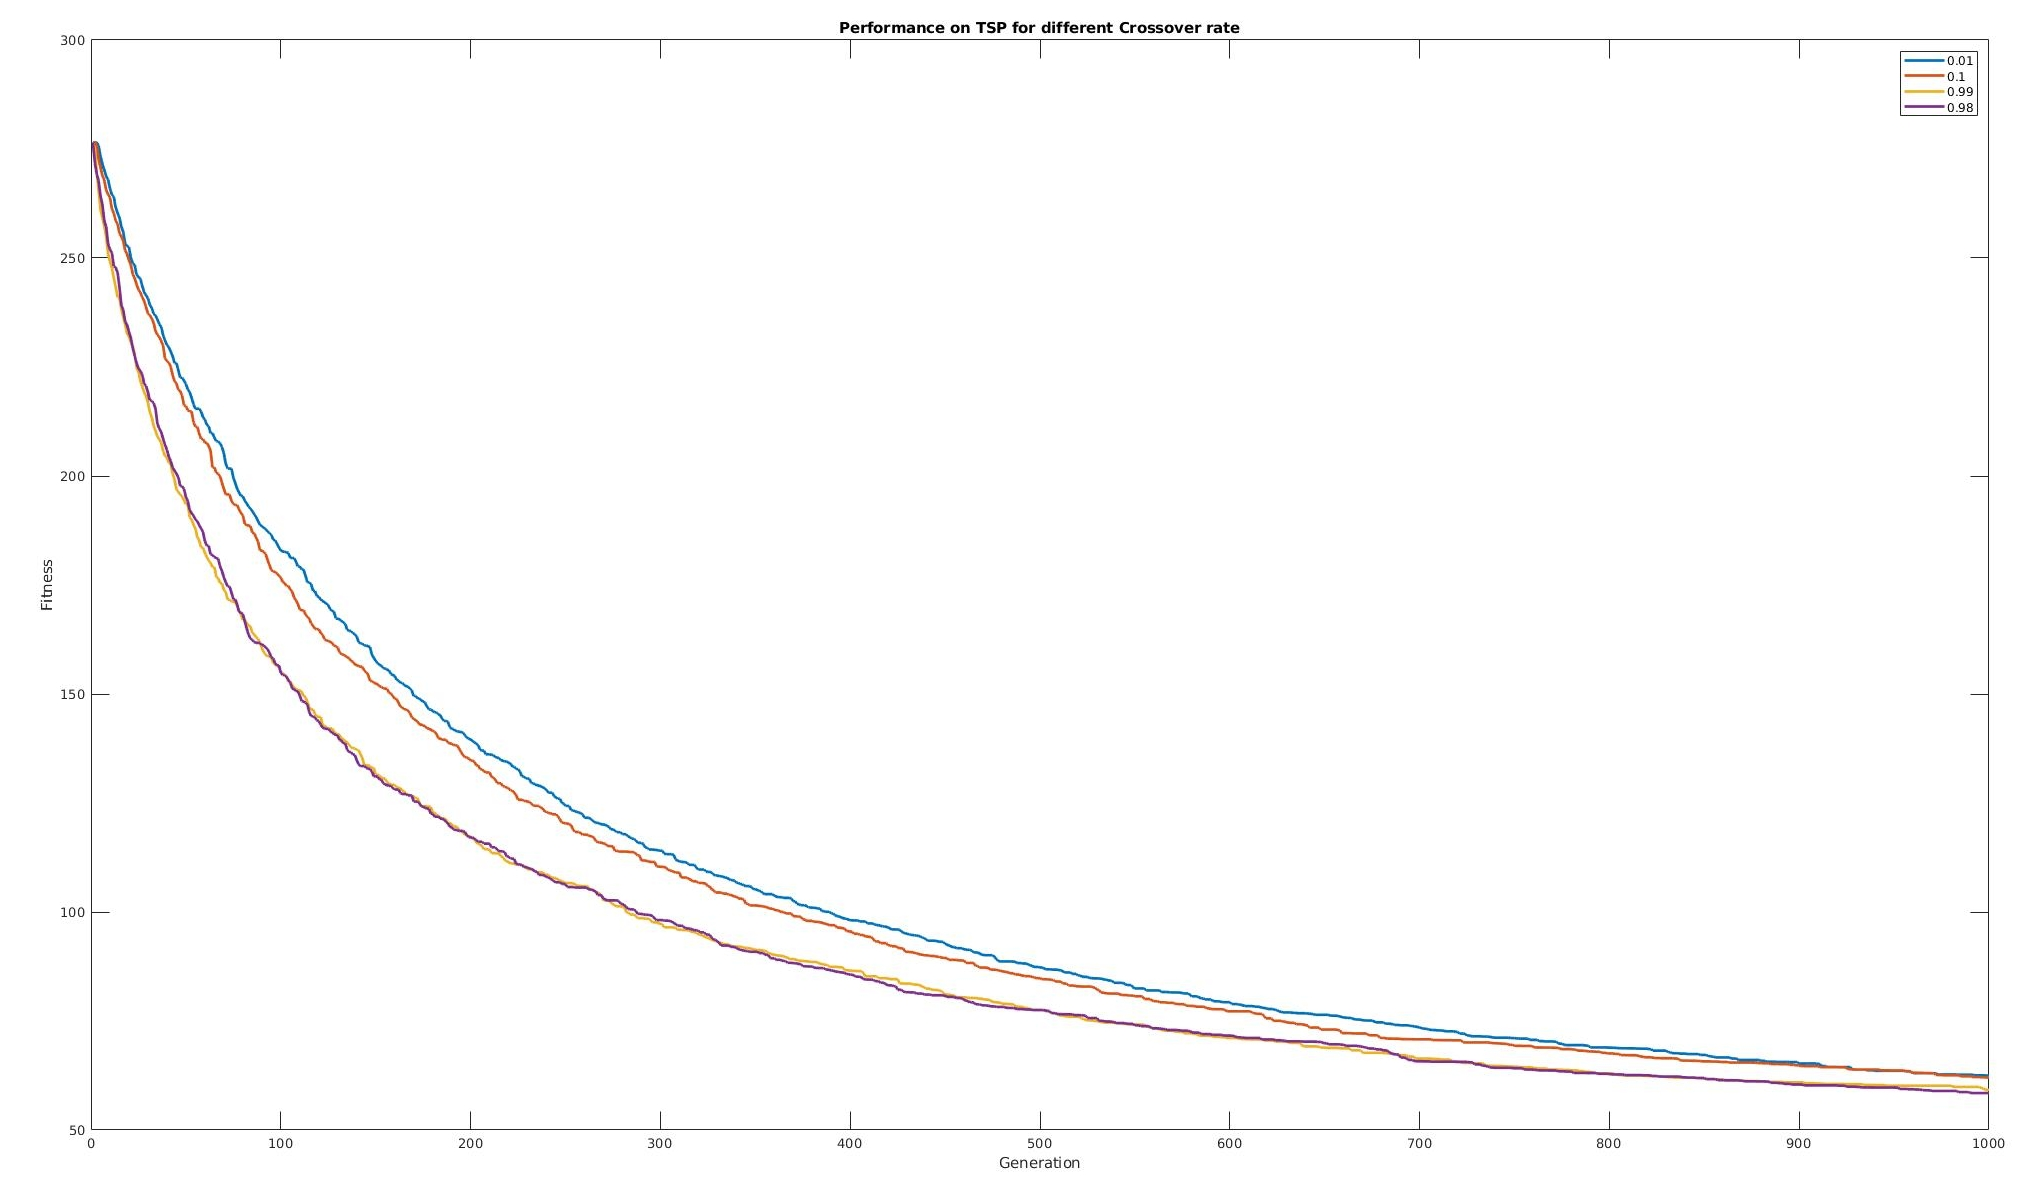
\includegraphics[width=1.0\textwidth]{images/crossover_exp_98.jpg}
	\caption{Crossover rate comparision\label{fig:crossfig}}
\end{figure}

\begin{itemize}
    \item We perform single point crossover.
    \item We choose \texttt{sp} individuals and select one with best fitness as father. We choose the mother in the same way.
    \item We select a \texttt{crossPoint} at random and select \texttt{1:crossPoint} genes from father's genotype and remaining available genes are added in the order in which they appear in mother's genotype.
    \item We have discovered that crossover rate of 98\% performs best over 1000 generations.
    \item As the crossover rate increases, the means fitness becomes better and better. This is expected, because when the rate is high, the child will have higher chance of being better than its parents but when the rate is low, child will probably be just a copy of father.
    \item As it is seen in Figure~\ref{fig:crossfig}, 98\% crossover rate experiment performs almost same with 99\% but slightly better at the very end of 1000 generations.
\end{itemize}

\newpage

\subsection{Different mutation rates}


\begin{figure}[ht!]
  \centering
  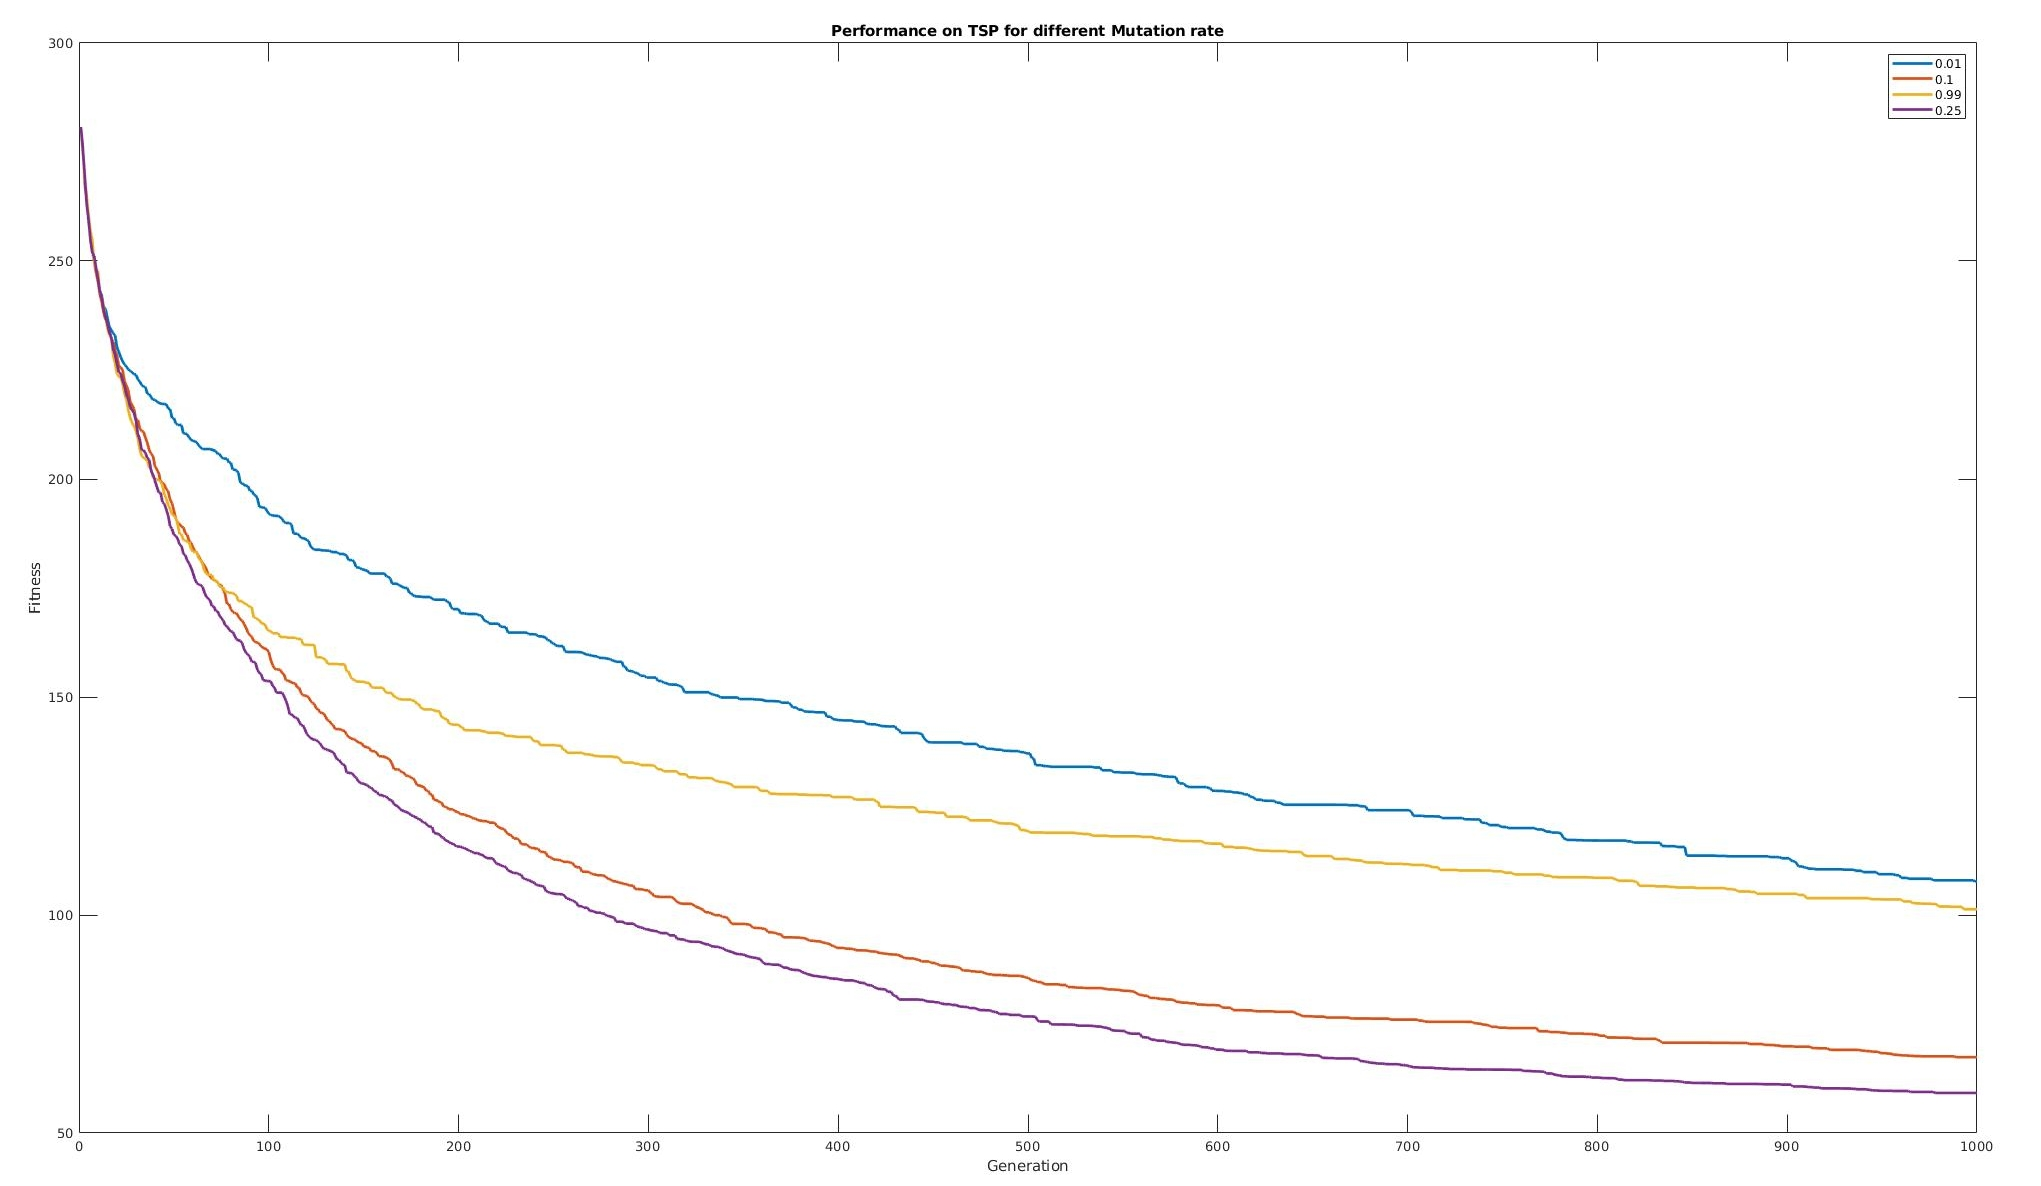
\includegraphics[width=1.0\textwidth]{images/mutation_exp_25.jpg}
    \caption{Mutation rate comparision\label{fig:mutfig}}
\end{figure}

\begin{itemize}
    \item We perform \textit{partial shuffle mutation}.
    \item We mutate an individual with \texttt{mutProb} probability.
    \item We select two points \textit{i,j}. We reverse the gene string between \textit{i} and \textit{j} and retain the parts of the gene string before \textit{i} and after \textit{j}.
    \item We have discovered that mutation rate of 25\% performs best over 1000 generations.
    \item From the experiment the choice of mutation rate of 25\% seems to be optimal over 1000 generations. If the rate is higher than 25\% then it disrupts the progress made till that generation and if it is lower than 25\% then it doesn't edit the gene string enough to show substantial progress.
    \item As seen from Figure~\ref{fig:mutfig}, mutation rate of 25\% performs best from the beginning till end of 1000 generations.
\end{itemize}

\newpage
\subsection{Best and median fitness variation over 30 experiments}
\begin{figure}[ht!]
  \centering
  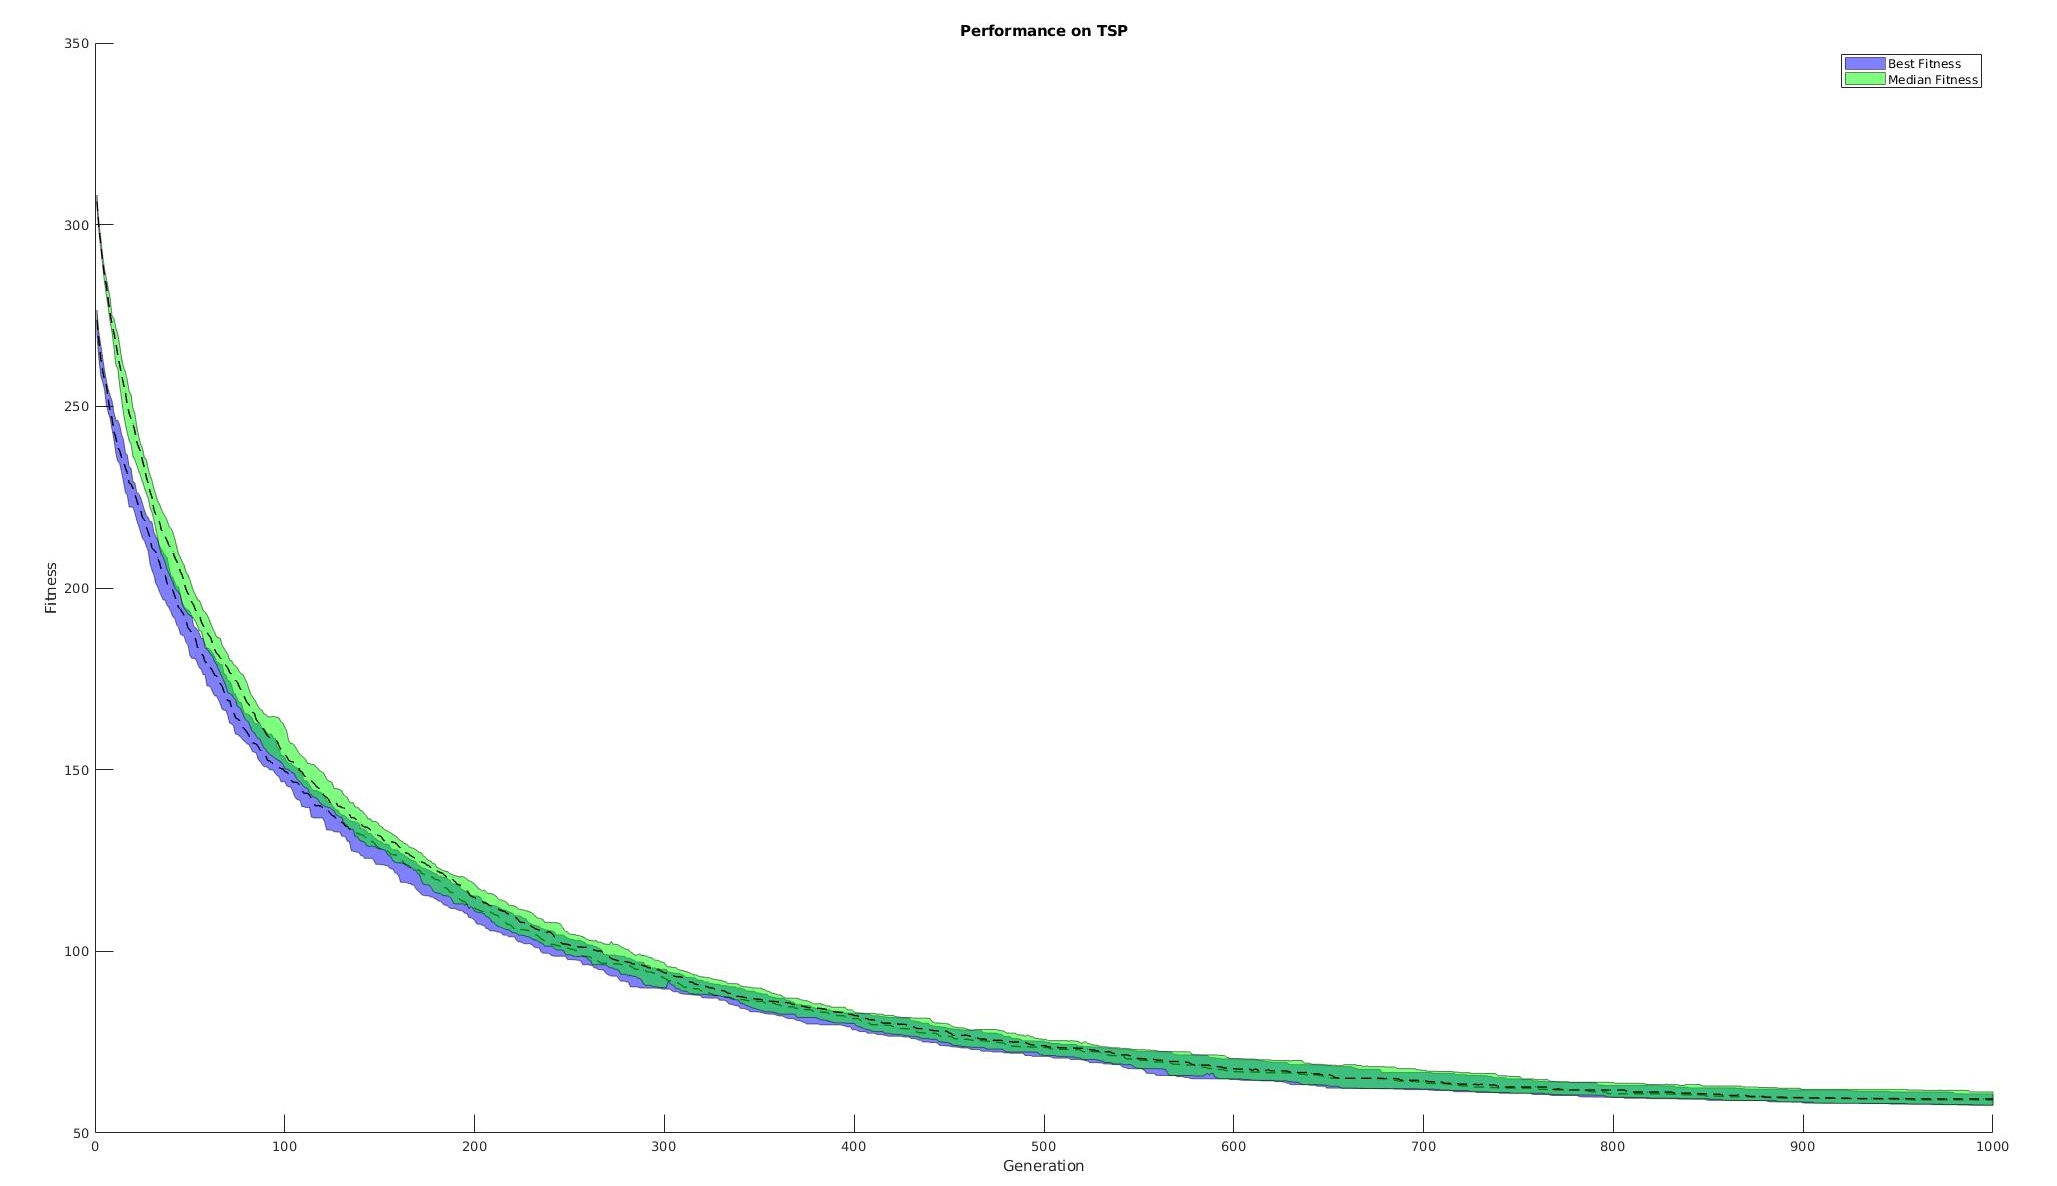
\includegraphics[width=1.0\textwidth]{images/1000X30_updated.jpg}
  \caption{Best and median fitness over 30 Experiments\label{fig:plot}}
\end{figure}

\newpage
\section{Comparision between absolute best for different generation}
\begin{figure}[ht!]
    \centering
    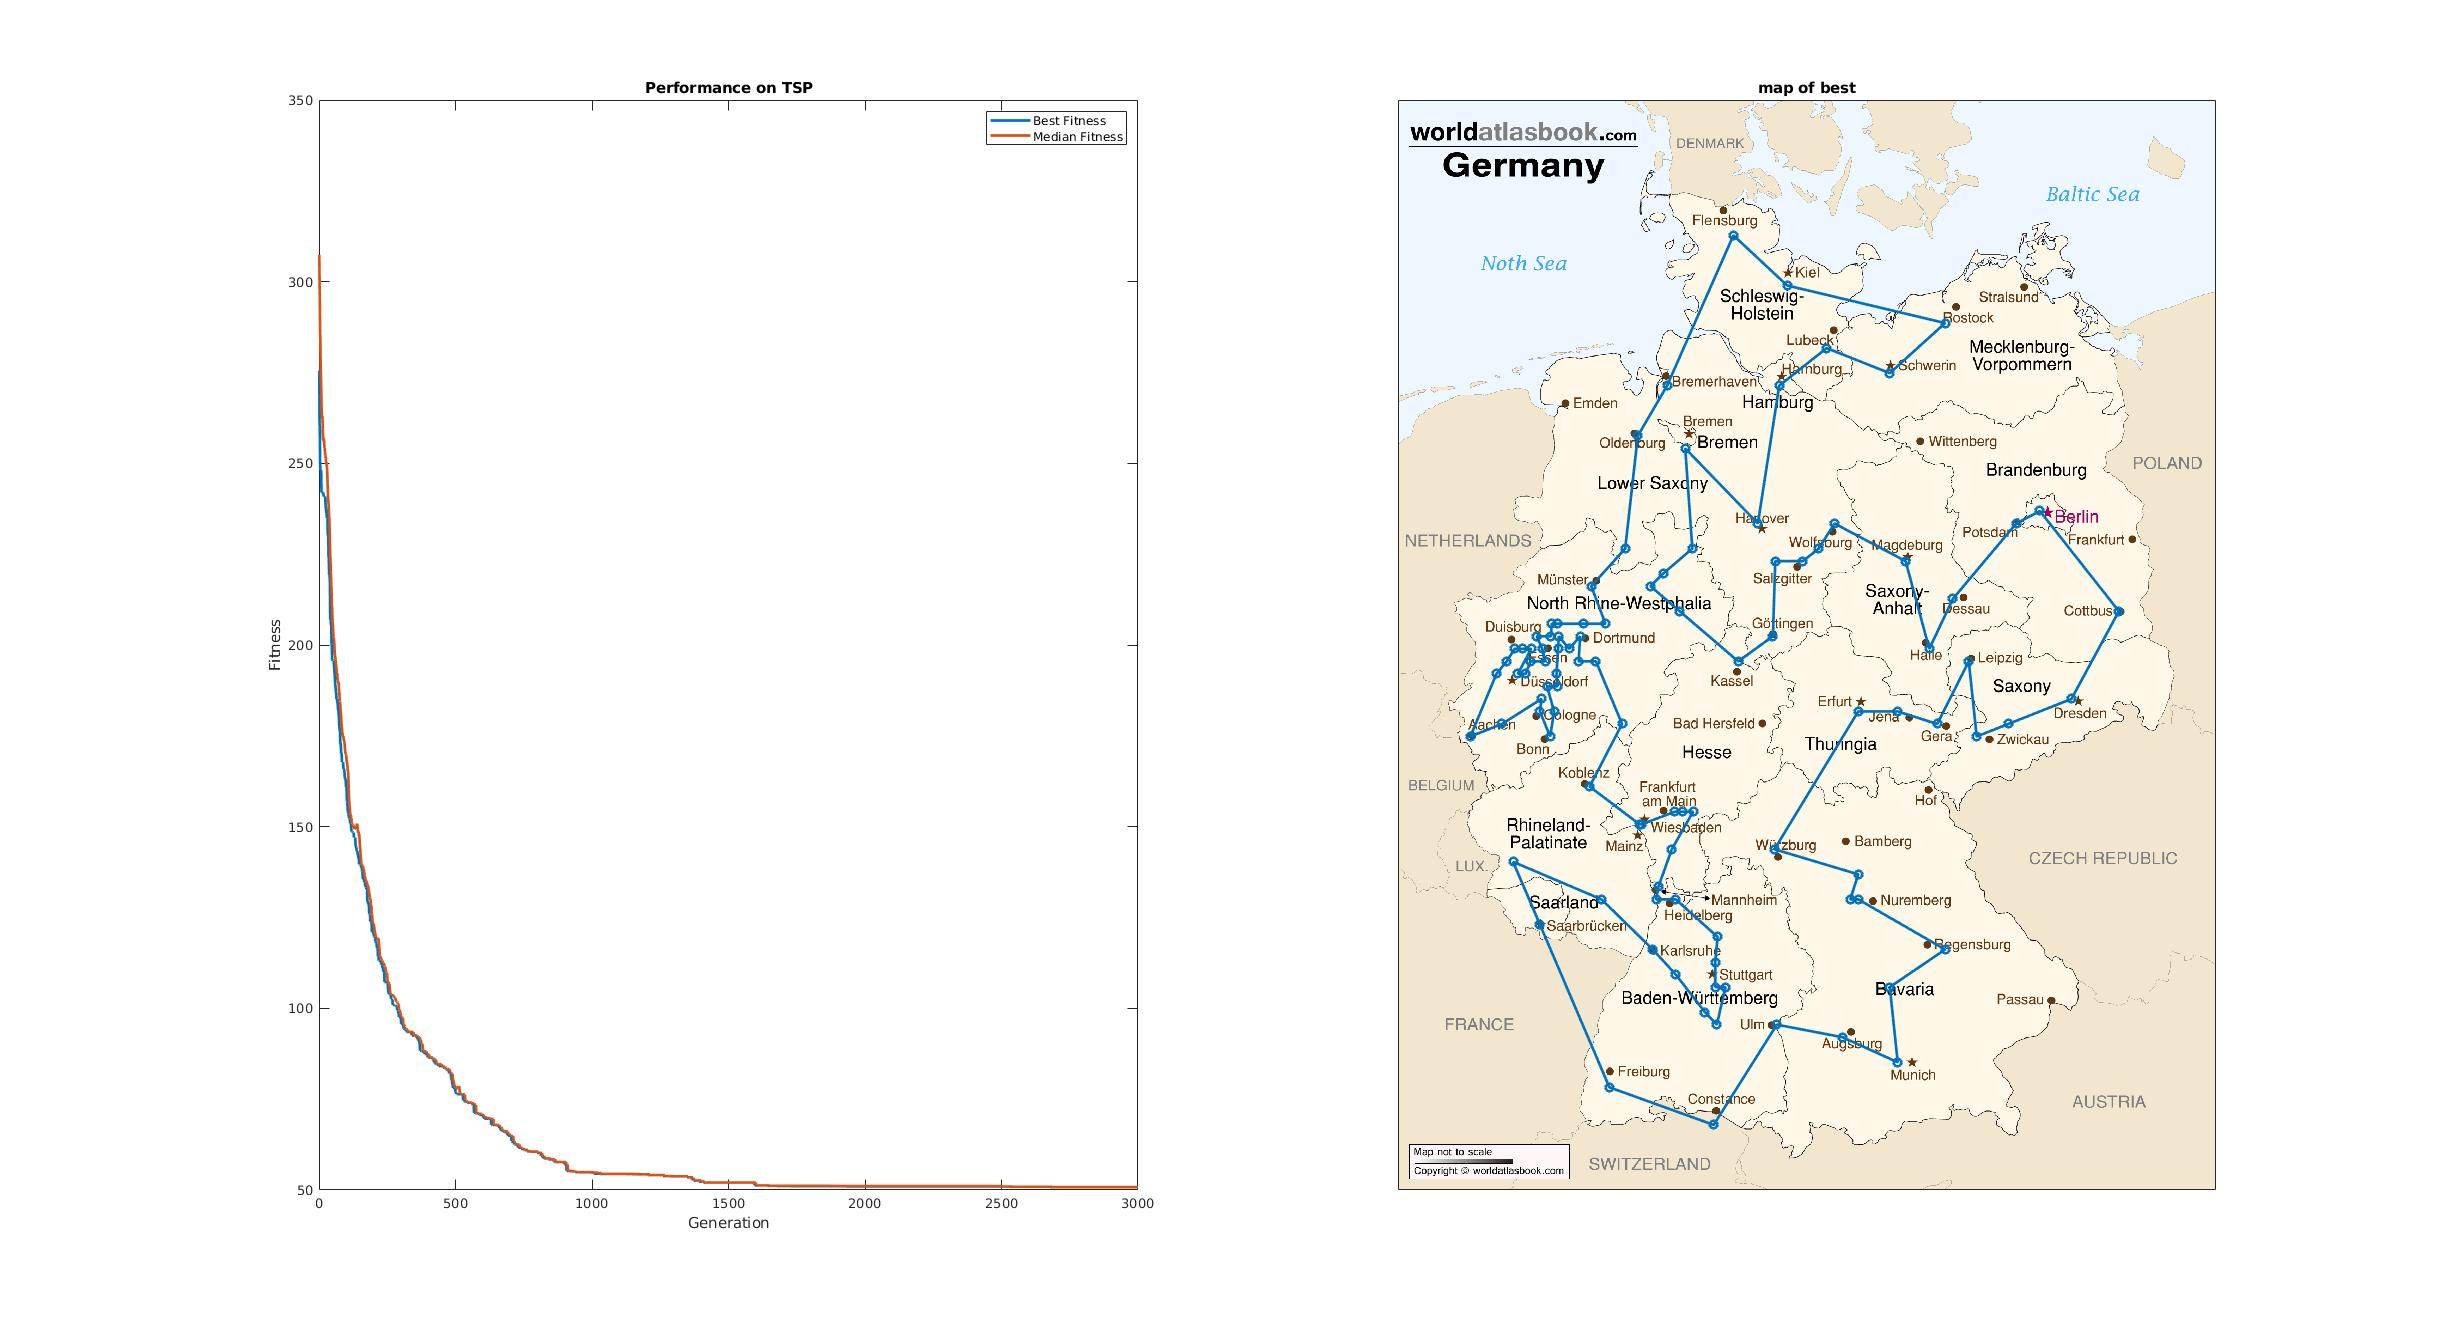
\includegraphics[width=1.0\linewidth]{images/BestPath_with_fitness.jpg}
    \caption{Plot and map for experiment over 3000 generations}
    \label{fig:plotAndMap3000}
\end{figure}

\begin{figure}[ht!]
    \centering
    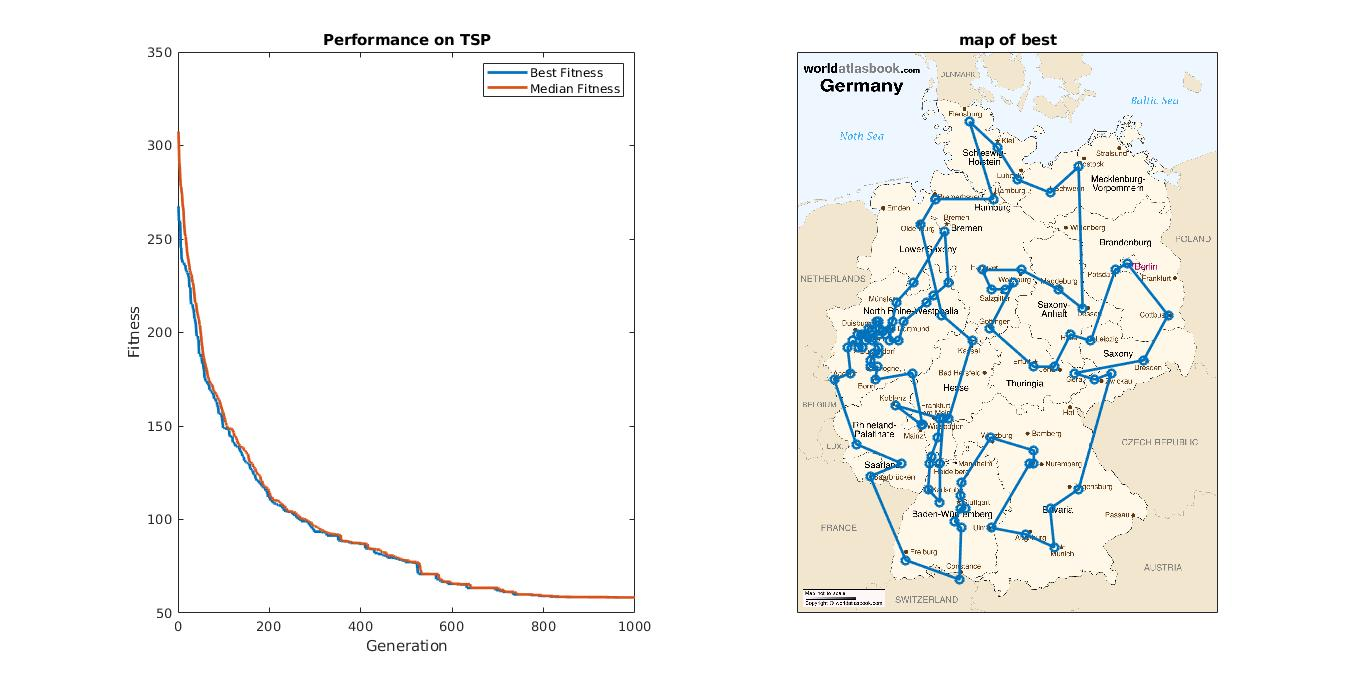
\includegraphics[width=1.0\linewidth]{images/BestPath_with_fitness_1000.jpg}
    \caption{Plot and map for experiment over 1000 generations}
    \label{fig:plotAndMap1000}
\end{figure}
\end{document}
